Community detection\ignore{, also know as clustering,} is the problem of uncovering the underlying structure of complex networks, i.e., identifying groups of vertices that exhibit dense internal connections but sparse connections with the rest of the network, in an unsupervised manner. It is an NP-hard problem with numerous applications in domains such as drug discovery, protein annotation, topic discovery, anomaly detection, and criminal identification. Communities identified are intrinsic when based on network topology alone, and are disjoint when each vertex belongs to only one community \cite{com-gregory10}.\ignore{One of the difficulties in the community detection problem is the lack of apriori knowledge on the number and size distribution of communities \cite{com-blondel08}.} The \textit{Louvain} method \cite{com-blondel08} is a popular heuristic-based approach for community detection, with the modularity metric \cite{com-newman06} being used to measure the quality of communities identified.

In recent years, the collection of data and the relationships among them, represented as graphs, have reached unmatched levels. This has necessitated the design of efficient parallel algorithms for community detection on large networks. The multicore/shared memory setting is crucial for community detection due to its energy efficiency and the prevalence of hardware with extensive DRAM sizes.\ignore{Optimizing parallel community detection algorithms for modern hardware architectures can yield notable performance benefits and competitive advantages across applications.} However, many of the current algorithms for community detection are challenging to parallelize due to their irregular and inherently sequential nature \cite{com-halappanavar17}, in addition to the complexities of handling concurrency, optimizing data access, reducing contention, minimizing load imbalance. Existing studies on Louvain propose algorithmic optimizations and parallelization techniques, but do not address optimization for the aggregation phase of the Louvain algorithm, which emerges as a bottleneck after the local-moving phase of the algorithm has been optimized. Moreover, these optimization techniques are scattered over a number of papers, making it difficult for a reader to get a grip over them.




\subsection{Our Contributions}

This report introduces GVE-Louvain, an optimized parallel implementation of Louvain\footnote{https://github.com/puzzlef/louvain-communities-openmp} for shared memory multicores. On a machine with two 16-core Intel Xeon Gold 6226R processors, GVE-Louvain outperforms Vite, Grappolo, and NetworKit Louvain by $50\times$, $22\times$, and $20\times$ respectively, achieving a processing rate of $560 M$ edges/s on a $3.8 B$ edge graph. With doubling of threads, GVE-Louvain exhibits an average performance scaling of $1.6\times$.




%% - Use --- for a dash.
%% - Use ``camera-ready'' for quotes.
%% - Use {\itshape very} or \textit{very} for italicized text.
%% - Use \verb|acmart| or {\verb|acmart|} for mono-spaced text.
%% - Use \url{https://capitalizemytitle.com/} for URLs.
%% - Use {\bfseries Do not modify this document.} for important boldface details.
%% - Use \ref{fig:name} for referencing.

%% For a block of pre-formatted text: 
% \begin{verbatim}
%   \renewcommand{\shortauthors}{McCartney, et al.}
% \end{verbatim}

%% For a list of items:
% \begin{itemize}
% \item the ``ACM Reference Format'' text on the first page.
% \item the ``rights management'' text on the first page.
% \item the conference information in the page header(s).
% \end{itemize}

%% For a table:
% \begin{table}
%   \caption{Frequency of Special Characters}
%   \label{tab:freq}
%   \begin{tabular}{ccl}
%     \toprule
%     Non-English or Math&Frequency&Comments\\
%     \midrule
%     \O & 1 in 1,000& For Swedish names\\
%     $\pi$ & 1 in 5& Common in math\\
%     \$ & 4 in 5 & Used in business\\
%     $\Psi^2_1$ & 1 in 40,000& Unexplained usage\\
%   \bottomrule
% \end{tabular}
% \end{table}

%% For a full-width table:
% \begin{table*}
%   \caption{Some Typical Commands}
%   \label{tab:commands}
%   \begin{tabular}{ccl}
%     \toprule
%     Command &A Number & Comments\\
%     \midrule
%     \texttt{{\char'134}author} & 100& Author \\
%     \texttt{{\char'134}table}& 300 & For tables\\
%     \texttt{{\char'134}table*}& 400& For wider tables\\
%     \bottomrule
%   \end{tabular}
% \end{table*}


%% For inline math:
% \begin{math}
%   \lim_{n\rightarrow \infty}x=0
% \end{math},

%% For a numbered equation:
% \begin{equation}
%   \lim_{n\rightarrow \infty}x=0
% \end{equation}

%% For an unnumbered equation:
% \begin{displaymath}
%   \sum_{i=0}^{\infty} x + 1
% \end{displaymath}

%% For a figure:
% \begin{figure}[h]
%   \centering
%   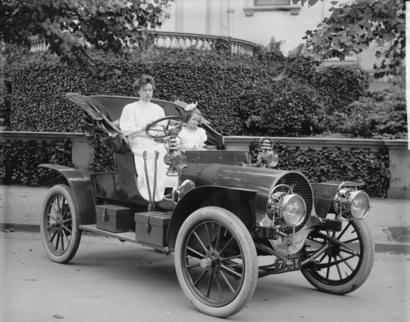
\includegraphics[width=\linewidth]{inc/sample-franklin}
%   \caption{1907 Franklin Model D roadster. Photograph by Harris \&
%     Ewing, Inc. [Public domain], via Wikimedia
%     Commons. (\url{https://goo.gl/VLCRBB}).}
%   \Description{A woman and a girl in white dresses sit in an open car.}
% \end{figure}

%% For a teaser figure.
% \begin{teaserfigure}
%   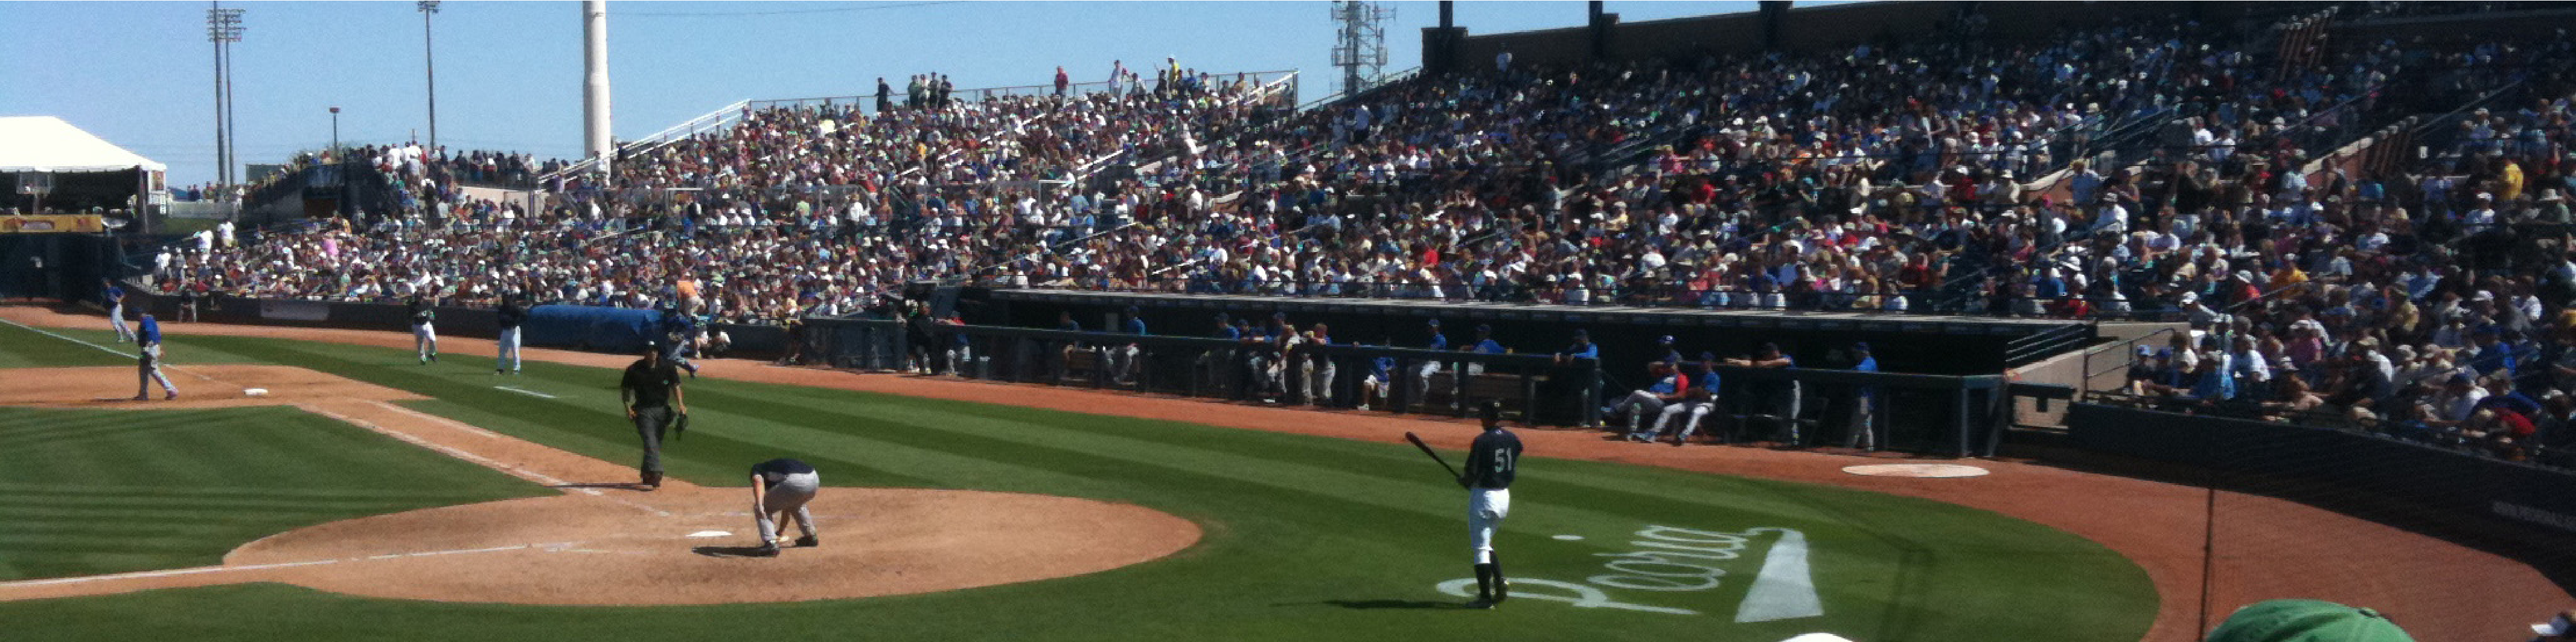
\includegraphics[width=\textwidth]{sampleteaser}
%   \caption{figure caption}
%   \Description{figure description}
% \end{teaserfigure}
